\chapter{Uso do simulador}
\label{chap:uso_simulador}

\lettrine{N}{este} capítulo explícase brevemente cómo empregar o simulador, explicando cómo xerar os arquivos .elf e empregar o simulador, así como interpretar o os resultados. 

O primeiro paso é empregar Segger Embedded Studio for RISC-V, aquí escribirase o código C para o programa. Antes de compilar, tendo seleccionado no panel esquerdo Project [Nome do proxecto], débese modificar en Project -> Compiler -> Elixir a extensión correcta, como se mostra na \ref{fig:cap1}. Por exemplo, no caso de que se realicen multiplicacións, débese cambiar de RV32I (por defecto) a RV32IM. Unha vez feito isto,  Build -> Build Solution. \ref{fig:compilar}
Agora na carpeta Output Files, están varios arquivos, entre eles o executable con extensión .elf.

Para o axuste parámetros debemos ir á Visual Studio 2022, no ficheiro config.h, aparecen definidas constante do tipo LatencyMul, como se ve na captura \ref{fig:parametros}.

\begin{figure}[hp!]
  \centering
  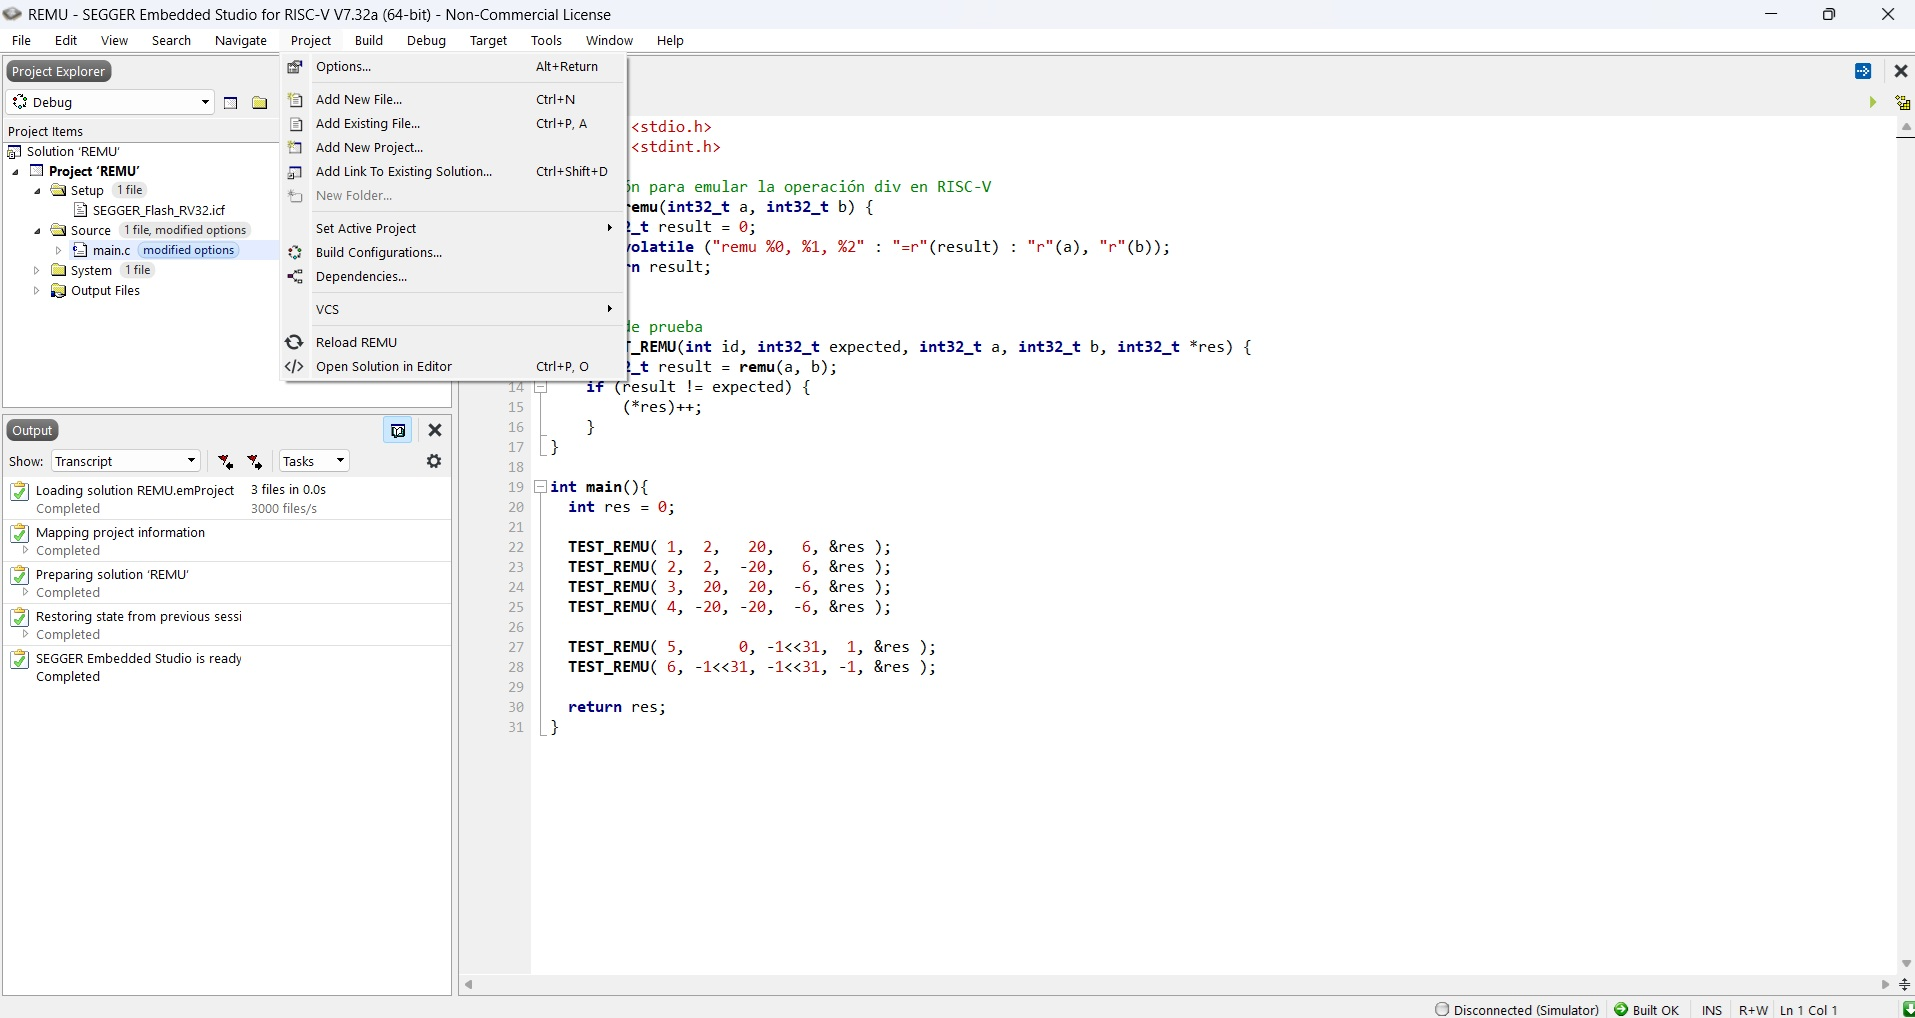
\includegraphics[width=\textwidth]{imaxes/Cap_1.jpg}
  \caption{Opcións do proxecto}
  \label{fig:cap1}
\end{figure}

\begin{figure}[hp!]
  \centering
  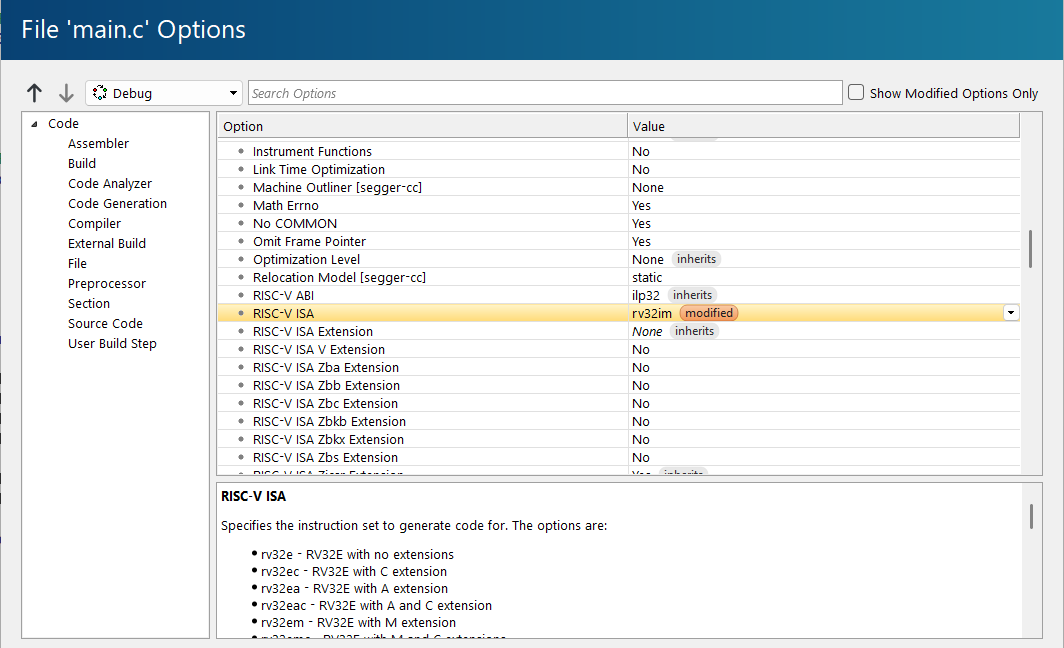
\includegraphics[width=\textwidth]{imaxes/Cap_2.png}
  \caption{Elección da extensión correcta}
  \label{fig:cap2}
\end{figure}


\begin{figure}[hp!]
  \centering
  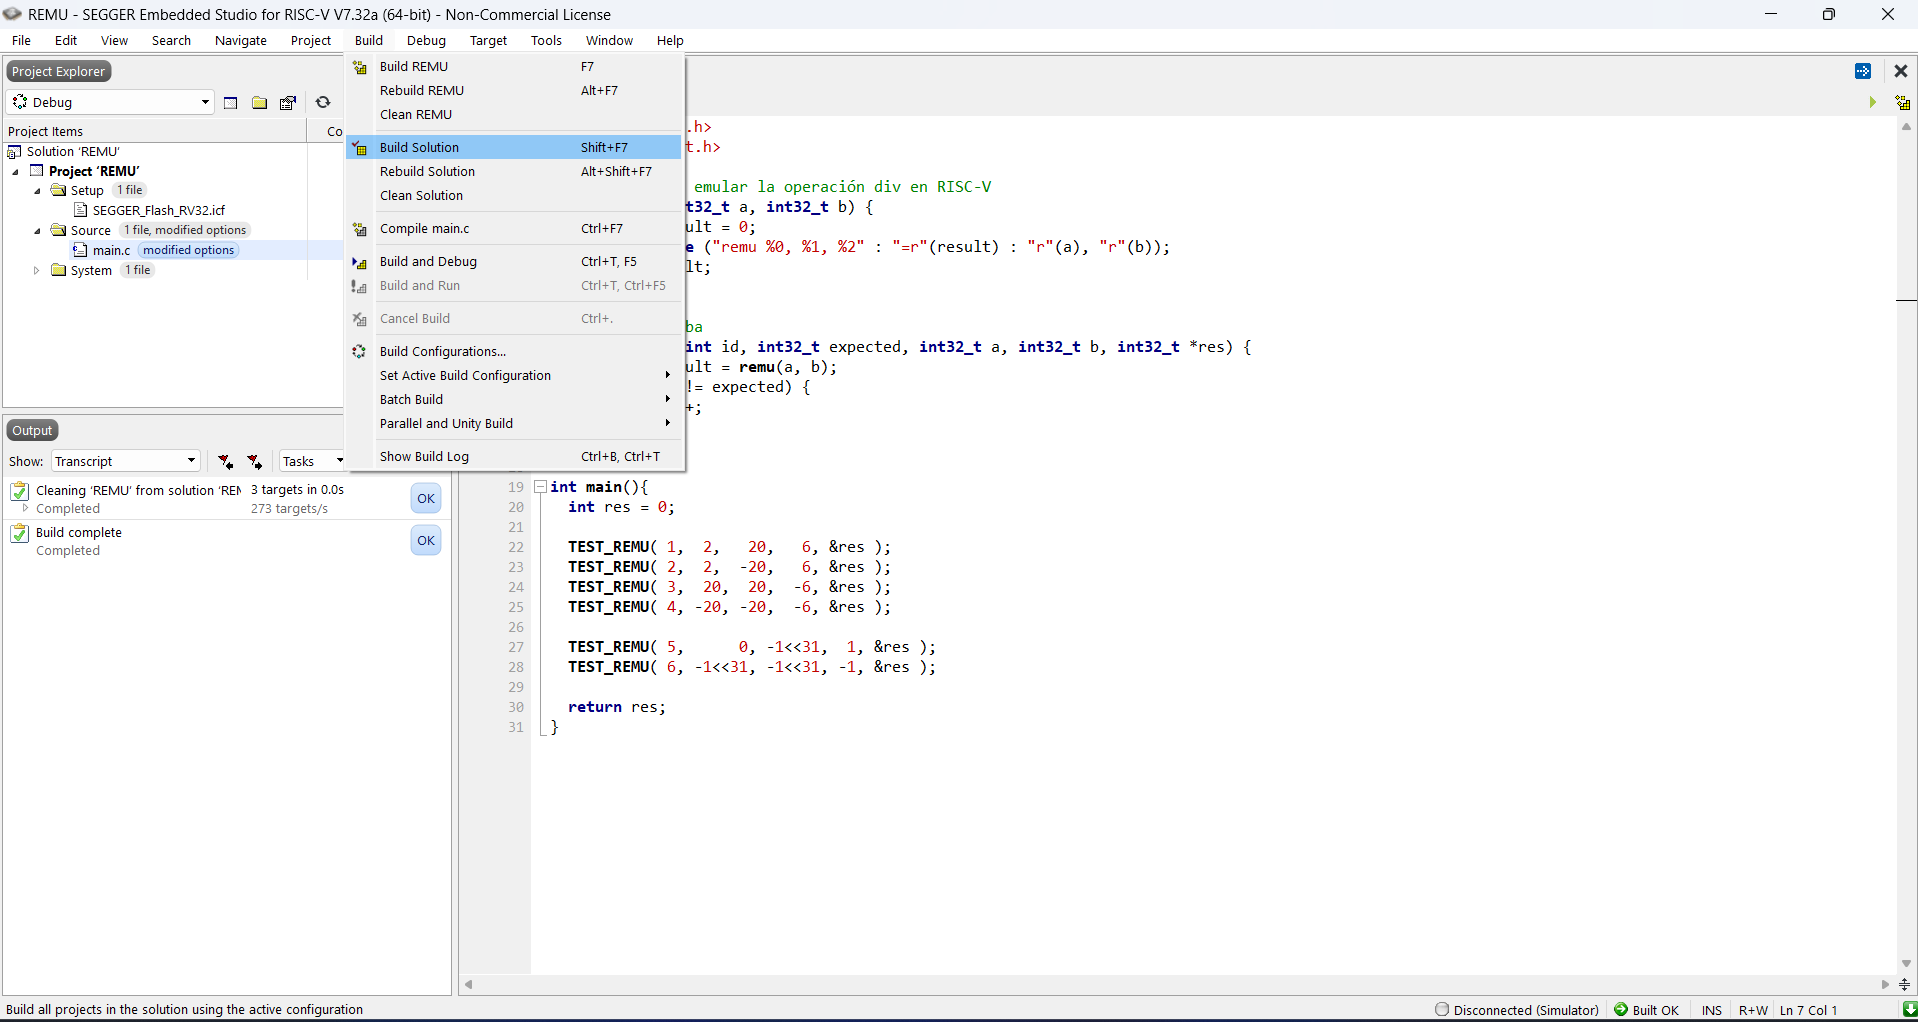
\includegraphics[width=\textwidth]{imaxes/Cap_3_Comp.png}
  \caption{Compilación do proxecto}
  \label{fig:compilar}
\end{figure}

\begin{figure}[hp!]
  \centering
  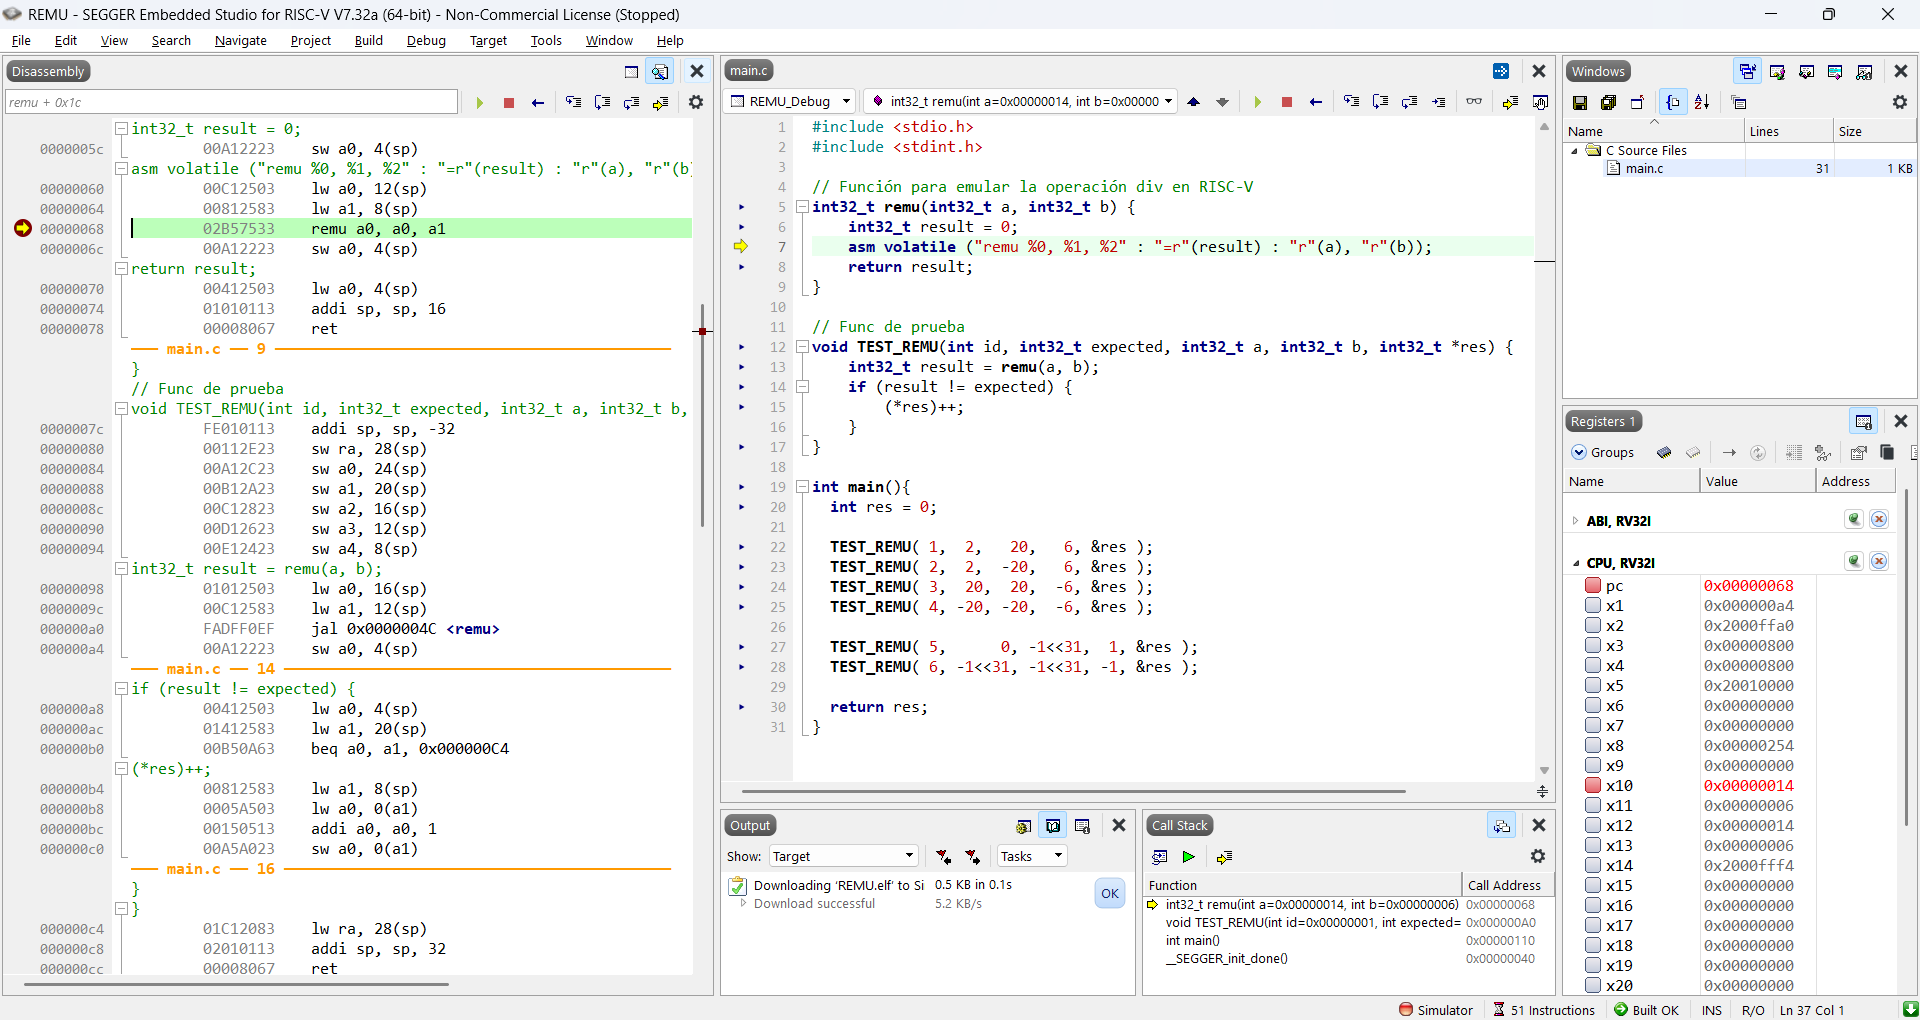
\includegraphics[width=\textwidth]{imaxes/Cap_4_Debug.png}
  \caption{Captura coas opcións de depuración de Segger}
  \label{fig:cap3}
\end{figure}

\begin{figure}[hp!]
  \centering
  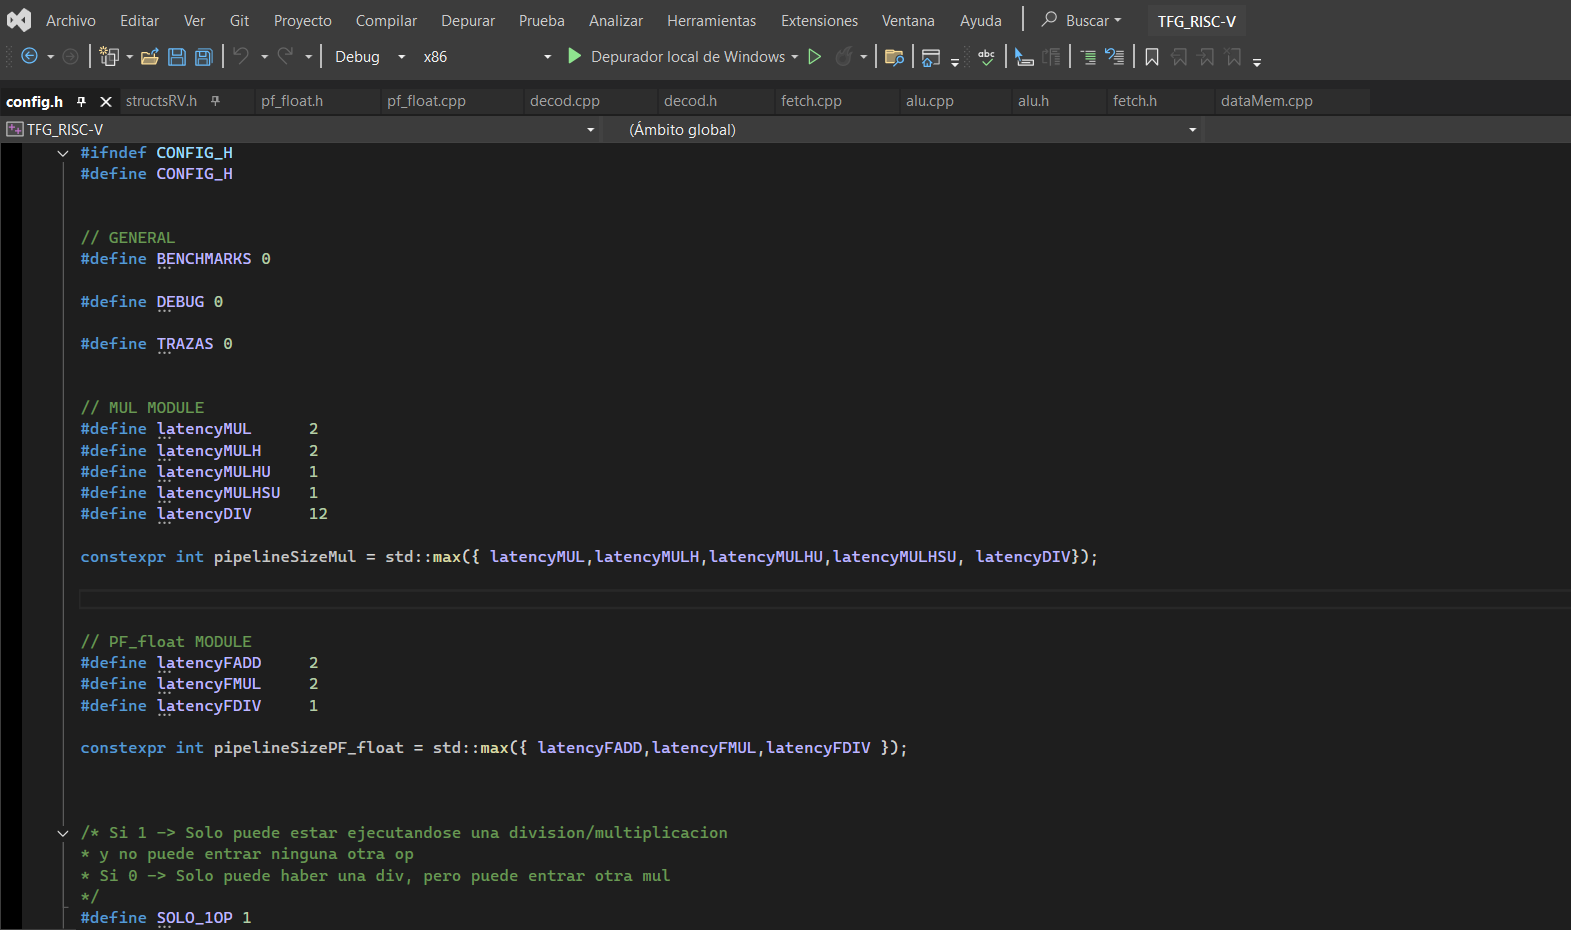
\includegraphics[width=\textwidth]{imaxes/Cap_5_Config.png}
  \caption{Cambio de parámetros en Config.h}
  \label{fig:parametros}
\end{figure}


\section{Resultados sobre a mellora do rendemento}\label{sec:rendemento}
Tras realizar varios test, pódese comprobar como varía o rendemento segundo a latencia elixida.



